\documentclass[8pt,a4paper,compress]{beamer}

\usepackage{/home/siyer/lib/slides}

\title{Programming Model}
\date{}

\begin{document}
\begin{frame}
\vfill
\maketitle
\end{frame}

\section{Basic Structure of a Java Program}
\begin{frame}[fragile]
\pause

The Java workflow

\smallskip

\begin{center}
\begin{tikzpicture}
\begin{scope}[->,xshift=-7.5cm,yshift=-5cm,thin,
	   node distance=1.6cm,on grid,>=stealth,
  	   block1/.style={rectangle,draw,align=center},
	   block2/.style={rectangle,align=center}]
\node [block1] (1) {editor \\ (Code)};
\node [block2] (2) [right=of 1] {\lstinline$P.java$};
\node [block1] (3) [right=of 2] {compiler \\ (\lstinline$javac$)};
\node [block2] (4) [right=of 3] {\lstinline$P.class$};
\node [block1] (5) [right=of 4] {JVM \\ (\lstinline$java$)};
\node [block2] (6) [right=of 5] {output};
\path (1) edge node [above] {} (2);
\path (2) edge node [above] {} (3);
\path (3) edge node [above] {} (4);
\path (4) edge node [above] {} (5);
\path (5) edge node [above] {} (6);
\end{scope}
\end{tikzpicture}
\end{center}

\pause\bigskip

A Java program is either a library of static methods (functions) or a data type definition

\pause\bigskip

To create a Java program (class), we use the following programming constructs
\begin{itemize}
\pause
\item Primitive data types and expressions

\pause
\item Statements

\pause
\item Arrays

\pause
\item Static methods

\pause
\item Strings

\pause
\item Input and output (IO)

\pause
\item Data abstraction
\end{itemize}
\end{frame}

\begin{frame}[fragile]
\pause

Example (Java program that computes $N!$)

\smallskip

\begin{lstlisting}[language=Java,style=focusin]
import edu.princeton.cs.algs4.StdOut;

public class Factorial {
    // Returns N!
    public static int factorial(int N) {
        int result = 1;
        for (int i = 1; i <= N; i++) {
            result *= i;
        }
        return result;
    }

    // Test client
    public static void main(String[] args) {
        int N = Integer.parseInt(args[0]);
        StdOut.println(N + "! = " + Factorial.factorial(N));
    }
}
\end{lstlisting}

\pause\bigskip

\begin{lstlisting}[language={},style=focusin]
$ javac Factorial.java
\end{lstlisting}

\pause\bigskip

\begin{lstlisting}[language={},style=focusin]
$ java Factorial 5
5! = 120
\end{lstlisting}
\end{frame}

\section{Primitive Data Types and Expressions}

\begin{frame}[fragile]
\pause

A data type (primitive or reference) is a set of values and a set of operations on those values

\pause\bigskip

Primitive types
\begin{itemize}
\pause
\item \lstinline{boolean}: true and false values with logical operations (\lstinline{!}, \lstinline{||}, and \lstinline{&&})

\pause
\item \lstinline{byte}: 8-bit integers with arithmetic operations (\lstinline{+}, \lstinline{-}, \lstinline{*}, \lstinline{/}, and \lstinline{%})

\pause
\item \lstinline{char}: 16-bit characters with arithmetic operations 

\pause
\item \lstinline{short}: 16-bit integers with arithmetic operations

\pause
\item \lstinline{int}: 32-bit integers with arithmetic operations

\pause
\item \lstinline{float}: 32-bit single-precision real numbers with arithmetic operations

\pause
\item \lstinline{long}: 64-bit integers with arithmetic operations

\pause
\item \lstinline{double}: 64-bit double-precision real numbers with arithmetic operations
\end{itemize}
\end{frame}

\begin{frame}[fragile]
\pause

An expression is a literal, a variable, or a sequence of allowed operations on literals and/or variables that produces a value

\pause\bigskip

Arithmetic operators \lstinline{*} and \lstinline{/} have higher precedence than \lstinline{+} and \lstinline{-}

\pause\bigskip

Among logical operators, \lstinline{!} has the highest precedence, followed by \lstinline{&&} and then \lstinline{||}

\pause\bigskip

Two operands of the same type can be compared using the relational operators \lstinline{==}, \lstinline{!=}, \lstinline{<}, \lstinline{<=}, \lstinline{>}, and \lstinline{>=}, producing a boolean result

\pause\bigskip

Relational operators have higher precedence than logical operators but lower precedence than arithmetic operators

\pause\bigskip

Operators of the same precedence are evaluated left to right

\pause\bigskip

Parentheses can be used to override precedence rules

\pause\bigskip

Numbers are automatically promoted to a more inclusive type

\pause\bigskip

A cast is a type name in parentheses within an expression, and converts the following value into a value of that type

\smallskip

\begin{lstlisting}[language=Java,style=focusin]
double x = (double) 42;
\end{lstlisting}
\end{frame}

\section{Statements}
\begin{frame}[fragile]
\pause

A statement defines computation by creating variables, assigning data-type values to them, and controlling the flow of execution

\pause\bigskip

A declaration statement associates a variable name with a type

\smallskip

\begin{lstlisting}[language={},style=focusin]
<type> <name>;
\end{lstlisting}

\smallskip

where the initial value for the variable is \lstinline{false} for boolean type, \lstinline{0} for numeric types, and \lstinline{null} for reference types

\pause\bigskip

An assignment statement associates a data-type value with a variable

\smallskip

\begin{lstlisting}[language={},style=focusin]
<name> = <expression>;
\end{lstlisting}

\pause\bigskip

Declaration and assignment statements can be combined to provide an initial value for a variable

\smallskip

\begin{lstlisting}[language={},style=focusin]
<type> <name> = <expression>;
\end{lstlisting}
\end{frame}

\begin{frame}[fragile]
\pause

A conditional statement is used when different actions are required for different inputs

\pause\bigskip

If statement

\smallskip

\begin{lstlisting}[language={},style=focusin]
if (<boolean expression>) {
    <statements>
}
else if (<boolean expression>) {
    <statements>
}
...
else {
    <statements>
}
\end{lstlisting}

\pause\bigskip

Conditional operator (really an expression)

\smallskip

\begin{lstlisting}[language={},style=focusin]
<boolean expression> ? <expression> : <expression>
\end{lstlisting}

\pause\bigskip

Switch statement

\smallskip

\begin{lstlisting}[language={},style=focusin]
switch (<expression>) {
    case <value>:
        <statements>
    case <value>:
        <statements>
    ...
    default:
        <statements>
}
\end{lstlisting}
\end{frame}

\begin{frame}[fragile]
\pause

A loop statement is used for repetitive computations

\pause\bigskip

While statement

\smallskip

\begin{lstlisting}[language={},style=focusin]
while (<boolean expression>) {
    <statements>
}
\end{lstlisting}

\pause\bigskip

For statement

\smallskip

\begin{lstlisting}[language={},style=focusin]
for (<initialize>; <boolean expression>; <increment>) {
    <statements>
}
\end{lstlisting}

\pause\bigskip

Do-while statement

\smallskip

\begin{lstlisting}[language={},style=focusin]
do {
    <statements>
} while (<boolean expression>);
\end{lstlisting}

\pause\bigskip

A break statement immediately exits a loop without letting it run to completion; when used as the last statement in a switch case, exits the switch statement preventing ``fallthrough'' to the following case

\pause\bigskip

A continue statement skips to next iteration of a loop
\end{frame}

\begin{frame}[fragile]
\pause

A compound assignment statement is shorthand notation for modifying the value of a variable

\pause\bigskip

For example
\begin{itemize}
\pause
\item \lstinline{i += 5;} is equivalent to \lstinline{i = i + 5;}

\pause
\item \lstinline{i++;} is equivalent to \lstinline{i = i + 1;}

\pause
\item \lstinline{--i;} is equivalent to \lstinline{i = i - 1;}
\end{itemize}

\pause\bigskip

The scope of a variable is the statements that follow the declaration in the same block (marked by curly brackets) as the declaration
\end{frame}

\section{Arrays}
\begin{frame}[fragile]
\pause

An array stores a sequence of values that are all of the same type 

\pause\bigskip

Making an array in Java involves: declaring the array name and type; creating the array; and initializing the array values

\smallskip

\begin{lstlisting}[language=Java,style=focusin]
int[] a;
a = new int[10];
for (int i = 0; i < 10; i++) {
    a[i] = i;
}
\end{lstlisting}

\pause\bigskip

An array when declared is initialized to \lstinline{null}, and once created, each element is initialized to a default value based on the type of the array

\pause\bigskip

Initializing declaration

\smallskip

\begin{lstlisting}[language=Java,style=focusin]
int[] a = {1, 1, 2, 3, 5, 8, 13, 21, 34, 55};
String[] b = {"Sun", "Mon", "Tue", "Wed", "Thu", "Fri", "Sat"};
\end{lstlisting}

\pause\bigskip

Example (reversing an array in place)

\smallskip

\begin{lstlisting}[language=Java,style=focusin]
int N = a.length;
for (int i = 0; i < N / 2; i++) {
    double temp = a[i];
    a[i] = a[N - 1 - i];
    a[N - i - 1] = temp;
}
\end{lstlisting}
\end{frame}

\begin{frame}[fragile]
\pause

If we assign one array name to another (aliasing), then both refer to the same array

\pause\bigskip

A two-dimensional array in Java is an array of one-dimensional arrays, and may be ragged

\pause\bigskip

Initializing declaration for two-dimensional arrays

\smallskip

\begin{lstlisting}[language=Java,style=focusin]
int[][] I = {{1, 0, 0}, 
             {0, 1, 0}, 
             {0, 0, 1}};
\end{lstlisting}

\pause\bigskip

Example (matrix multiplication $C_{ij}=\sum_{k=1}^{p} A_{ik}B_{kj},$ where $A$ is an $m\times p$, $B$ is a $p \times n$, and $C$ is an $m\times n$ matrix)

\smallskip

\begin{lstlisting}[language=Java,style=focusin]
int m = A.length;
int p = B.length;
int n = B[0].length;
double[][] C = new double[m][n];
for (int i = 0; i < m; i++) {
    for (int j = 0; j < n; j++) {
        for (int k = 0; k < p; k++) {
            C[i][j] += A[i][k] * B[k][j];
        }
    }
}
\end{lstlisting}
\end{frame}

\section{Static Methods}
\begin{frame}[fragile]
\pause

A method encapsulates a computation defined as a sequence of statements

\pause\bigskip

A static method is composed of the keywords \lstinline{public static} followed by a return type (or \lstinline{void}), the signature (method name and a sequence of arguments, each with a declared type), and a body (a sequence of statements enclosed by curly brackets)

\pause\bigskip

Example (primality testing)

\smallskip

\begin{lstlisting}[language=Java,style=focusin]
public static boolean isPrime(int N) {
    if (N < 2) { return false; }
    for (int i = 2; i <= N / i; i++) { if (N % i == 0) { return false; } }
    return true;
}
\end{lstlisting}

\pause\bigskip

A call on a static method is its name followed by expressions that specify argument values in parentheses, separated by commas

\pause\bigskip

When a method call is part of an expression, the method computes a value and that value is used in place of the call in the expression

\pause\bigskip

Properties of methods
\begin{itemize}
\pause
\item Arguments are passed by value

\pause
\item Method names can be overloaded 

\pause
\item A method has a single return value but may have multiple return statements

\pause
\item A method can have side effects
\end{itemize}
\end{frame}

\begin{frame}[fragile]
\pause

A recursive method is one that calls itself, has a base case, addresses subproblems that are smaller in some sense, and does not address subproblems that overlap

\pause\bigskip

Example of good recursion (computing $N!$)
\[
N! = \begin{dcases*}
N(N-1)! & if $N > 0$, and \\
1       & if $N=0$
\end{dcases*}
\]

\smallskip

\begin{lstlisting}[language=Java,style=focusin]
public static int f(int N) {
    return (N == 0) ? 1 : N * f(N - 1); 
}
\end{lstlisting}

\pause\bigskip

Call trace for \lstinline{f(5)}

\smallskip

\begin{lstlisting}[language={},style=focusin]
f(5)
  f(4)
    f(3)
      f(2)
        f(1)
          f(0)
            return 1
          return 1 * 1 = 1            
        return 2 * 1 = 2
      return 3 * 2 = 6
    return 4 * 6 = 24
  return 5 * 24 = 120
\end{lstlisting}
\end{frame}

\begin{frame}[fragile]
\pause

Example of bad recursion (computing $N$th Fibonacci number)
\[
f(N) = \begin{dcases*}
f(N-1) + f(N-2) & if $N > 1$, and \\
1       & if $N=0$ or $N=1$
\end{dcases*}
\]

\smallskip

\begin{lstlisting}[language=Java,style=focusin]
public static int f(int N) {
    return (N == 0 || N == 1) ? 1 : f(N - 1) + f(N - 2); 
}
\end{lstlisting}

\pause\bigskip

Call trace for \lstinline{f(5)}
\begin{center}
\visible<3->{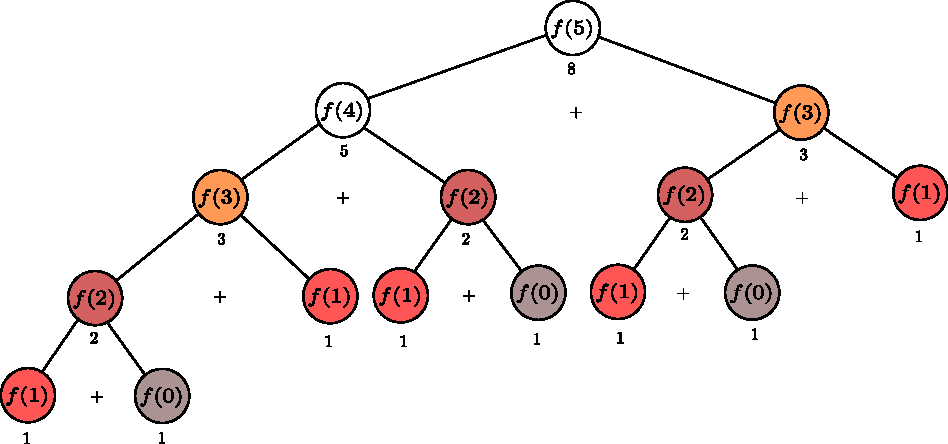
\includegraphics[scale=0.6]{figures/fib_trace.pdf}}
\end{center}
\end{frame}

\begin{frame}[fragile]
\pause

A best practice in Java programming is to include a \lstinline{main()} method (aka development or test client) in every library of static methods

\pause\bigskip

We use static methods from four different kinds of libraries
\begin{itemize}
\pause
\item Standard system libraries \lstinline{java.lang.*}

\pause
\item Imported system libraries such as \lstinline{java.util.Arrays}

\pause
\item Other libraries in the text

\pause
\item Standard libraries \lstinline{edu.princeton.cs.algs4.*} from the text
\end{itemize}
\end{frame}

\section{APIs}
\begin{frame}[fragile]
\pause

An application programming interface (API) lists the library name and the return type, signatures, and short descriptions of each of the methods

\pause\bigskip

A client is a program that calls a method in another library

\pause\bigskip

An implementation is Java code that implements the methods in an API

\pause\bigskip

Standard system library (\lstinline{java.lang.Math})
\begin{center}
\begin{tabular}{cc}
method & description \\ \hline
\lstinline$static double abs(double a)$  & $|a|$ \\
\lstinline$static double max(double a, double b)$  & $\max(a, b)$ \\
\lstinline$static double min(double a, double b)$  & $\min(a, b)$ \\
\lstinline$static double sin(double theta)$  & $\sin(\theta)$ \\
\lstinline$static double cos(double theta)$  & $\cos(\theta)$ \\
\lstinline$static double tan(double theta)$  & $\tan(\theta)$ \\
\lstinline$static double random()$ & $\text{real} \in [0, 1)$ \\
\lstinline$static double E$ & $e$ \\
\lstinline$static double PI$ & $\pi$ \\
$\dots$ & $\dots$ 
\end{tabular} 
\end{center}

\pause\bigskip

Imported system library (\lstinline{java.util.Arrays})
\begin{center}
\begin{tabular}{cc}
method & description \\ \hline
\lstinline$static void sort(int[] a)$ & put the array in ascending order \\
$\dots$ & $\dots$ 
\end{tabular} 
\end{center}
\end{frame}

\begin{frame}[fragile]
\pause

Standard libraries from the text
\begin{itemize}
\item \lstinline{edu.princeton.cs.algs4.StdRandom}
\begin{center}
\begin{tabular}{cc}
method & description \\ \hline
\lstinline$static void initialize(long seed)$ & initialize \\
\lstinline$static double random()$ & $\text{real} \in [0, 1)$ \\
\lstinline$static int uniform(int N)$ & $\text{integer} \in [0, N)$ \\
\lstinline$static int uniform(int lo, int hi)$ & $\text{integer} \in [lo, hi)$ \\
\lstinline$static double uniform(double lo, double hi)$ & $\text{real} \in [lo, hi)$ \\
\lstinline$static boolean bernoulli(double p)$ & \lstinline$true$ with probability $p$ \\
\lstinline$static double gaussian()$ & $\text{real} \in \mathcal{N}(0, 1)$ \\
\lstinline$static double gaussian(double m, double s)$ & $\text{real} \in \mathcal{N}(m, s)$ \\
\lstinline$static int discrete(double[] a)$ & $i$ with probability $a[i]$ \\
\lstinline$static void shuffle(double[] a)$ & shuffle the array \\
$\dots$ & $\dots$ 
\end{tabular} 
\end{center}

\item \lstinline{edu.princeton.cs.algs4.StdStats}
\begin{center}
\begin{tabular}{cc}
method & description \\ \hline
\lstinline$static double max(double[] a)$ & largest value \\
\lstinline$static double min(double[] a)$ & smallest value \\
\lstinline$static double mean(double[] a)$ & average \\
\lstinline$static double var(double[] a)$ & sample variance \\
\lstinline$static double stddev(double[] a)$ & sample standard deviation \\
\lstinline$static double median(double[] a)$ & median \\
$\dots$ & $\dots$ 
\end{tabular} 
\end{center}
\end{itemize}
\end{frame}

\section{Strings}
\begin{frame}[fragile]
\pause

A string is a sequence of characters (\lstinline{char} values) 

\pause\bigskip

A string literal is a sequence of characters within double quotes, such as \lstinline{"Hello, World"}

\pause\bigskip

The result of concatenating two strings using the \lstinline{+} operator is a single string, the first string followed by the second

\pause\bigskip

We use Java library methods such as \lstinline{Integer.parseInt()}, \lstinline{Double.parseDouble()}, and so on to convert strings to primitives

\pause\bigskip

We use the \lstinline{+} operator to convert primitives to strings
\end{frame}

\section{Input and Output}
\begin{frame}[fragile]
\pause

Bird's-eye biew of a Java program
\begin{center}
\begin{tikzpicture}
\begin{scope}[->,xshift=-7.5cm,yshift=-5cm,thin,
	   node distance=1.6cm,on grid,>=stealth,
  	   block1/.style={rectangle,draw,align=center},
	   block2/.style={rectangle,align=center}]
\node [block2] (1) {input};
\node [block1] (2) [right=of 1] {\lstinline{P.java}};
\node [block2] (3) [right=of 2] {output};
\path (1) edge node [above] {} (2);
\path (2) edge node [above] {} (3);
\end{scope}
\end{tikzpicture}
\end{center}

\pause\bigskip

Input types: command-line arguments, standard input, file input

\pause\bigskip

Output types: standard output, file output

\pause\bigskip

Command-line arguments are listed after the program name as follows

\smallskip

\begin{lstlisting}[language={},style=focusin]
$ java P arg_1 arg_2 ... arg_n
\end{lstlisting}

\smallskip

and accessed within the \lstinline$main()$ method of the program via the array \lstinline$args$  as \lstinline$args[0]$, \lstinline$args[1]$, $\dots$, \lstinline$args[n - 1]$

\pause\bigskip

Example

\smallskip

\begin{lstlisting}[language=Java,style=focusin]
import edu.princeton.cs.algs4.StdOut;

public class UseArgument {
    public static void main(String[] args) {
        StdOut.print("Hi, ");
        StdOut.print(args[0]);
        StdOut.println(". How are you?");
    }
}
\end{lstlisting}

\pause\bigskip

\begin{lstlisting}[language={},style=focusin]
$ java UseArgument Alice
Hi, Alice. How are you?
\end{lstlisting}

\pause\bigskip

\begin{lstlisting}[language={},style=focusin]
$ java UseArgument Bob
Hi, Bob. How are you?
\end{lstlisting}
\end{frame}

\begin{frame}[fragile]
\pause

Standard output (\lstinline{edu.princeton.cs.algs4.StdOut}) API
\begin{center}
\begin{tabular}{cc}
method & description \\ \hline
\lstinline$static void println(String s)$ & print $s$, followed by a newline \\
\lstinline$static void printf(String f, ...)$ & formatted print \\
$\dots$ & $\dots$ 
\end{tabular} 
\end{center}

\pause\bigskip

Example

\smallskip

\begin{lstlisting}[language=Java,style=focusin]
import edu.princeton.cs.algs4.StdOut;
import edu.princeton.cs.algs4.StdRandom;

public class RandomSeq {
    public static void main(String[] args) { 
        int N = Integer.parseInt(args[0]);
        double lo = Double.parseDouble(args[1]);
        double hi = Double.parseDouble(args[2]);
        for (int i = 0; i < N; i++) {
            double x = StdRandom.uniform(lo, hi);
            StdOut.printf("%.2f\n", x);
        }
    }
}
\end{lstlisting}

\pause\bigskip

\begin{lstlisting}[language={},style=focusin]
$ java RandomSeq 2 100.0 200.0
193.12
190.79
\end{lstlisting}
\end{frame}

\begin{frame}[fragile]
\pause

Standard input (\lstinline{edu.princeton.cs.algs4.StdIn}) API
\begin{center}
\begin{tabular}{cc}
method & description \\ \hline
\lstinline$static boolean isEmpty()$ & \lstinline$true$ if no more values, \lstinline$false$ otherwise \\
\lstinline$static int readInt()$ & read a value of type \lstinline$int$ \\
\lstinline$static double readDouble()$ & read a value of type \lstinline$double$ \\
$\dots$ & $\dots$ 
\end{tabular} 
\end{center}

\pause\bigskip

Example

\smallskip

\begin{lstlisting}[language=Java,style=focusin]
import edu.princeton.cs.algs4.StdIn;
import edu.princeton.cs.algs4.StdOut;

public class Average { 
    public static void main(String[] args) { 
        int count = 0; 
        double sum = 0.0;
        while (!StdIn.isEmpty()) {
            double value = StdIn.readDouble();
            sum += value;
            count++;
        }
        double average = sum / count;
        StdOut.println("Average is " + average);
    }
}
\end{lstlisting}

\pause\bigskip

\begin{lstlisting}[language={}]
$ java Average
1 2 3 4 5
<ctrl-d>
Average is 3.0
\end{lstlisting}
\end{frame}

\begin{frame}[fragile]
\pause

Output redirection

\smallskip

\begin{lstlisting}[language={},style=focusin]
$ java RandomSeq 1000 100.0 200.0 > data.txt
\end{lstlisting}

\pause\smallskip

\begin{lstlisting}[language={},style=focusin]
$ head -5 data.txt
155.83
191.65
197.83
191.90
111.84
\end{lstlisting}

\pause\bigskip

Input redirection

\smallskip

\begin{lstlisting}[language={},style=focusin]
$ java Average < data.txt
Average is 149.1812199999999
\end{lstlisting}

\pause\bigskip

Piping

\smallskip

\begin{lstlisting}[language={},style=focusin]
$ java RandomSeq 1000 100.0 200.0 | java Average
Average is 150.0588699999999
\end{lstlisting}
\end{frame}
\end{document}
